\section{Interpretable Invariances by Null-Sampling}\label{ssec:general}
% \begin{figure}
%     \centering
%     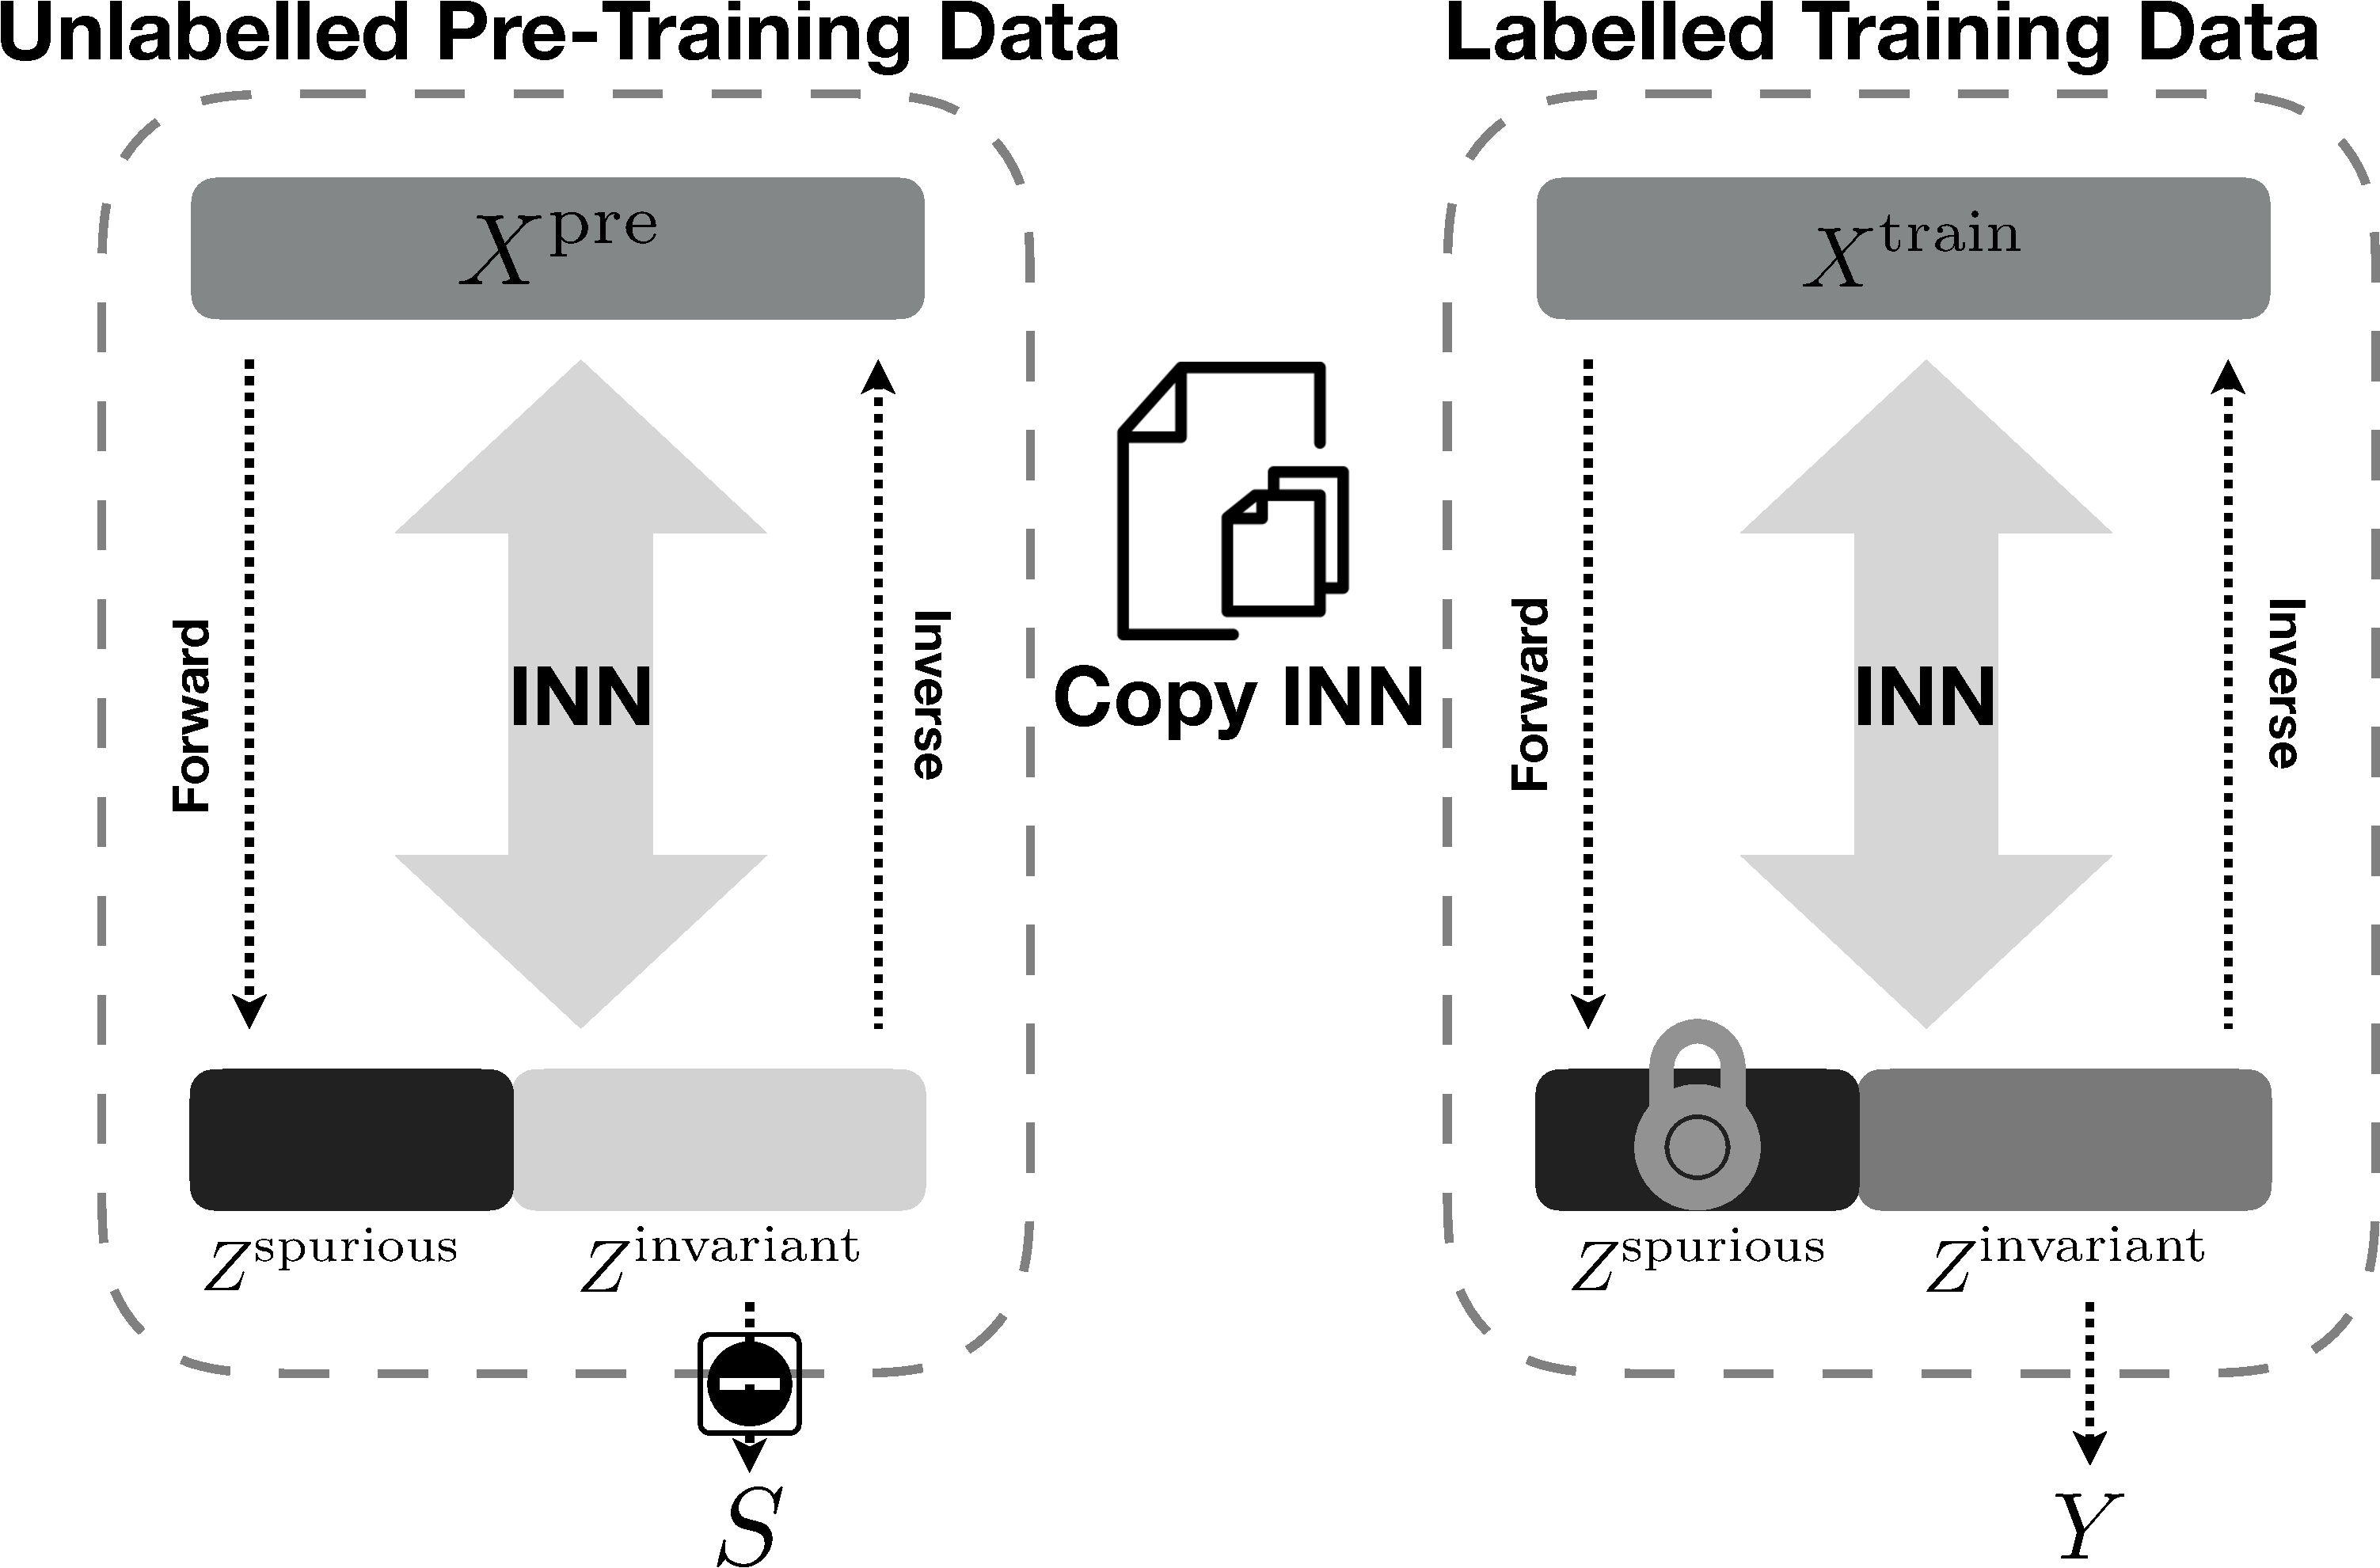
\includegraphics[width=0.4\textwidth]{./Figures/diagram.pdf}
%     \caption{Training procedure using the cFlow model for illustrative purposes.}%
%     \label{fig:training_diagram}
% \end{figure}
\begin{figure*}[tb]
    \centering
    \hfill
    \subfloat[cFlow model.]{%
        \scalebox{0.33}{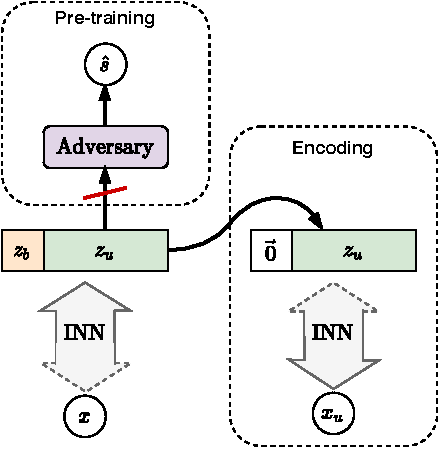
\includegraphics[width=\textwidth]{./Figures/inn_diagram_u.pdf}}%
        \label{fig:inn_diagram}
    }
    \hfill
    \subfloat[cVAE model.]{%
        \scalebox{0.4}{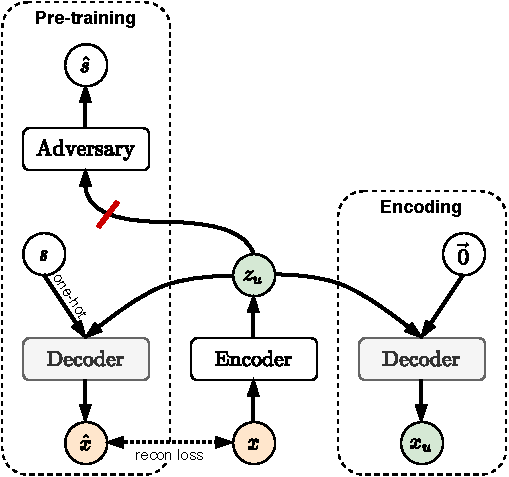
\includegraphics[width=\textwidth]{./Figures/cvae_diagram_u.pdf}}%
        \label{fig:cvae_diagram}
    }
    \hfill
    \caption{
        Training procedure for our models. $x$: input, $s$: sensitive attribute, $z_u$: de-biased representation, $x_u$: de-biased version of the input in the data domain.
        The red bar indicates a gradient reversal layer, and $\stackrel{\rightarrow}{0}$ the null-sampling operation.
    }%
    \label{fig:model-diagrams}
\end{figure*}

\subsection{Problem Statement} % HEADING IS JUST TO HELP ORGANIZE THOUGHTS, WILL BE DELETED LATER
\noindent We assume we are given inputs $\bm{x} \in \mathcal{X}$ and corresponding labels $y \in \mathcal{Y}$.
Furthermore, there is some spurious variable $s \in \mathcal{S}$ associated with each input $\bm{x}$ which we do \emph{not} want to predict. 
Let $X$, $S$ and $Y$ be random variables that take on the values $\bm{x}$, $s$ and $y$, respectively.
The fact that both $y$ and $s$ are predictive of $\bm{x}$ implies that $\mathcal{I}(X;Y), \mathcal{I}(X;S) > 0$, where $\mathcal{I}(\cdot ;\cdot)$ is the mutual information.
Note, however, that the conditional entropy is non-zero: $H(S|X) \neq 0$, i.e., $S$ is not completely determined by $X$.

%The difficulty emerges in the construction of the fully-supervised training dataset in which correspondence between $S$ and $Y$ is exaggerated compared to the test set.
The difficulty of this setup emerges in the training set: there is a close correspondence between $S$ and $Y$, such that for a model that sees the data through the lens of the loss function, the two are indistinguishable.
Furthermore, we assume that this is \emph{not} the case in the test set, meaning the model cannot rely on shortcuts provided by $S$ if it is to generalise from the training set.

We call this scenario where we only have access to the labels of a biasedly-sampled subpopulation
an \emph{aggravated fairness problem}.
These are not uncommon in the real-world.
For instance, in long-feedback systems such as mortgage-approval where the demographics of the subpopulation with observed outcomes is \emph{not} representative of the subpopulation on which the model has been deployed. 
In this case, $s$ has the potential to act as a false (or \emph{spurious}) indicator of the class label and
training a model with such a dataset would limit generalisability.
Let $(X^\mathit{tr}, S^\mathit{tr}, Y^\mathit{tr})$ then be the random variables sampled for the training set
and $(X^\mathit{te}, S^\mathit{te}, Y^\mathit{te})$ be the random variables for the test set.
The training and test sets thus induce the following inequality for their mutual information:
$\mathcal{I}(S^\mathit{tr}; Y^\mathit{tr}) \gg \mathcal{I}(S^\mathit{te}; Y^\mathit{te}) \approx 0$.

% \subsection{In an Ideal World} % HEADING IS JUST TO HELP ORGANIZE THOUGHTS, WILL BE DELETED LATER
Our goal is to learn a representation $\bm{z}_u$ that is independent of $s$ and transferable between downstream tasks.
Complementary to $\bm{z}_u$, we refer to some abstract component of the model that absorbs the unwanted information related to $s$ as $\mathcal{B}$, the realisation of which we define with respect to each of the two models to be described.
%To satisfy this objective, we introduce an additional regularisation term
%that can be viewed from an information-theoretic perspective as minimising the mutual information between the random variables:
The requirement for $\bm{z}_u$ can be expressed via mutual information:
\begin{align}
  I(\bm{z}_u;s) \overset{!}{=} 0~.
  \label{eq:migoal}
\end{align}
However, for the representation to be useful, we need to capture as much relevant information in the data as possible.
Thus, the combined objective function:
\begin{align}
  \min_{\theta} \mathbb{E}_{x \sim X}[-\log p_\theta(\bm{x})] + \lambda I(f_\theta(x);s)
  \label{eq:objectivetheory}
\end{align}
where $\theta$ refers to the trainable parameters of our model $f_\theta$ and $p_\theta(\bm{x})$ is the likelihood it assigns to the data.

We optimise this loss in an adversarial fashion by playing a min-max game, in which our encoder acts as the generative component.
The adversary is an auxiliary classifier $g$, which receives $\bm{z}_u$ as input and attempts to predict the spurious variable $s$.
We denote the parameters of the adversary as $\phi$;
for the parameters of the encoder we use $\theta$, as before.
The objective from~\eqref{eq:objectivetheory} is then% realised as
\begin{align}
  \min_{\theta\in\Theta} \max_{\phi\in\Phi} \mathbb{E}_{x \sim X}[\log p_\theta(x) -\lambda\mathcal{L}_c(g_\phi(f_\theta(x))); s)]
  \label{eq:objectivepractical}
\end{align}
where $\mathcal{L}_c$ is the cross-entropy between the predictions for $s$ and the provided labels.
In practice, this adversarial term is realised with a gradient reversal layer (GRL) \citep{ganin2016domain} between $\bm{z}_u$ and $g$ as is common in adversarial approaches~\citep{edwards2016censoring}.
% to fair representation learning

\subsection{The Disentanglement Dilemma} % HEADING IS JUST TO HELP ORGANIZE THOUGHTS, WILL BE DELETED LATER
The objective in~\eqref{eq:objectivepractical} balances the two desiderata: predicting $y$ and being invariant to $s$.
However, in the training set $(X^\mathit{tr}, S^\mathit{tr}, Y^\mathit{tr})$,
$y$ and $s$ are so strongly correlated that removing information about $s$ inevitably removes information about $y$.
This strong correlation makes existing methods fail under this setting.
% However, this objective is complicated by the desideratum that $\bm{z}_u$ remain predictive of $y$,
% which precludes us from directly training on the target-labelled dataset $(X^\mathit{tr}, S^\mathit{tr}, Y^\mathit{tr})$,
%where $y$ and $s$ are so strongly correlated that removing information about $s$ inevitably removes information about $y$.
%We therefore need
In order to even define the right learning goal,
we require another source of information that allows us to disentangle $s$ and $y$.
For this, we assume the existence of another set of samples that follow a similar distribution to the test set,
but whilst the sensitive attribute is available, the class labels are not.
In reality, this is not an unreasonable assumption,
as, while properly annotated data is scarce, unlabelled data can be obtained in abundance (with demographic information from census data, electoral rolls, etc.).
Previous work has also considered treated ``unlabelled data'' as still having $s$ labels~\citep{wick2019unlocking}.
We are restricted only in the sense that the spurious correlations we want to sever are indicated in the features.
We call this the \emph{representative set}, consisting of $X^\mathit{rep}$ and $S^\mathit{rep}$.
It fulfils $\mathcal{I}(S^\mathit{rep}; Y^\mathit{rep}) \approx 0$
(or rather, it would, if the class labels $Y^\mathit{rep}$ were available).
%{\color{red} justify the existence of such a dataset}

We now summarise the training procedure; an outline for the invertible network model (cFlow) can be seen in fig.~\ref{fig:inn_diagram}.
First, the encoder network $f$ is trained on ($X^\mathit{rep}, S^\mathit{rep}$), during the first phase.
The trained network is then used to encode the training set,
taking in $\bm{x}$ and producing the representation, $\bm{z}_u$, decorrelated from the spurious variable.
The encoded dataset can then be used to train any off-the-shelf classifier safely, with information about the spurious variable having been absorbed by some auxiliary component $\mathcal{B}$.
In the case of the conditional VAE (cVAE) model,
$\mathcal{B}$ takes the form of the decoder subnetwork, which reconstructs the data conditional on a one-hot encoding of $s$,
while for the invertible network $\mathcal{B}$ is realised as a partition of the feature map $\bm{z}$
(such that $\bm{z} = [\bm{z}_u, \bm{z}_b]$), given the bijective constraint.
Thus, the classifier cannot take the shortcut of learning $s$ and instead must learn how to predict $y$ directly.
Obtaining the $s$-invariant representations, $\bm{x}_u$, in the data domain
is simply a matter of replacing the $\mathcal{B}$ component of the decoder's input for the cVAE,
and $\bm{z}_b$ for cFlow, with a zero vector of equivalent size.
We refer to this procedure used to generate $\bm{x}_u$ as \emph{null-sampling} (here, with respect to $\bm{z}_b)$.

% This That said, we do wish to draw a distinction between null-sampling and the annihilation operation featured in .
Null-sampling resembles the \emph{annihilation} operation described in \citet{xiao2017dna}, however we note that the two serve very different roles.  Whereas the annihilation operation serves as a regulariser to prevent trivial solutions (similar to \cite{jaiswal2018unsupervised}), null-sampling is used to generate the invariant representations post-training.

\subsection{Conditional Decoding}%
\label{conddec}
\noindent We first describe a VAE-based model similar to that proposed in~\citet{madras2018learning}, before highlighting some of its shortcomings that motivate the choice of an invertible representation learner.

The model takes the form of a class conditional $\beta$-VAE \citep{higgins2017beta}, in which the decoder is conditioned on the spurious attribute.
We use $\theta_{enc}, \theta_{dec} \in \theta$ to denote the parameters of the encoder and decoder sub-networks, respectively.
Concretely, the encoder component performs the mapping $x \rightarrow{\bm{z}_u}$, while $\mathcal{B}$ is instantiated as the decoder,
$\mathcal{B} \coloneqq p_{\theta_{dec}}(x|z_u, s)$, which takes in a concatenation of the learned non-spurious latent vector $\bm{z}_u$ and a one-hot encoding of the spurious label $s$ to produce a reconstruction of the input $\hat{x}$.
Conditioning on a one-hot encoding of $s$, rather than a single value, as done in \citet{madras2018learning} is the key to visualising invariant representations in the data domain.
If $\mathcal{I}(z_u; s)$ is properly minimised, the decoder can only derive its information about $s$ from the label, thereby freeing up $\bm{z}_u$ from encoding the unwanted information while still allowing for reconstruction of the input.
Thus, by feeding a zero-vector to the decoder we achieve $\hat{x} \perp s$.
The full learning objective for the cVAE is given as
\begin{align}
\begin{split}
    \mathcal{L}_{\mathrm{cVAE}} =& \mathbb{E}_{q_{\theta_{enc}}(z_u, b|x)}[\log p_{\theta_{dec}}(x|z, b) - \log p_{\theta_{dec}}(s|z_u)] \\ 
    &- \beta D_{KL}(q_{\theta_{enc}}(z_u |x) \| p(z_u))
\end{split}
\end{align}
where $\beta$ is a hyperparameter that determines the trade-off between reconstruction accuracy and independence constraints,
and $p(\bm{z}_u)$ is the prior imposed on the variational posterior.
For all our experiments, $p(\bm{z}_u)$ is realised as an Isotropic Gaussian.
Fig.~\ref{fig:cvae_diagram} summarises the procedure as a diagram.

While we show this setup can indeed work for simple problems, as~\citet{madras2018learning} before us have, we show that it lacks scalability due to disagreement between the components of the loss.
Since information about $s$ is only available to the decoder as a binary encoding,
if the relationship between $s$ and $x$ is highly non-linear and cannot be summarised by a simple on/off mechanism, as is the case if $s$ is an attribute such as gender,
off-loading information to the decoder by conditioning is no longer possible. As a result, $\bm{z}_u$ is forced to carry information about $s$ in order to minimise the reconstruction error. 

The obvious solution to this is to allow the encoder to store information about $s$ in a partition of the latent space as in  \citet{creager2019flexibly}.  However, we question whether an autoencoder is the best choice for this setup, with the view that an invertible model is the better tool for the task. Using an invertible model has several guarantees, namely complete information-preservation and freedom from a reconstruction loss, the importance of which we elaborate on below.

\subsection{Conditional Flow}\label{cflow}
\paragraph{Invertible Neural Networks.}
Invertible neural networks are a class of neural network architecture characterised by a bijective mapping between their inputs and output \citep{Dinh2014}. The transformations are designed such that their inverses and Jacobians are efficiently computable.
These flow-based models permit \emph{exact} likelihood estimation \citep{normflows2015} through the warping of a base density with a series of invertible transformations and computing the resulting, highly multi-modal, but still normalised, density, using the change of variable theorem:
% Flow-GAN \cite{grover2018flowgan} combines the \emph{exact} log-likelihood estimation of the invertible network with the adversarial training of a GAN.
\begin{align}
\begin{split}
  \log p(x) &= \log p(z) + 
   \sum \log \left| \det\left( \frac{\diff h_i}{ h_{i-1}}\right) \right|, %\\
  \quad p(z) = \mathcal{N}(z; 0, \mathbb{I})
  \label{eq:changeofvariables}
\end{split}
\end{align}
where $h_i$ refers to the outputs of the layers of the network and $p(z)$ is the base density, specifically an Isotropic Gaussian in our case.
Training of the invertible neural network is then reduced to maximising $\log p(x)$ over the training set,
i.e.\ maximising the probability the network assigns to samples in the training set.

% The requirement of analytic invertibility and Jacobians demands the use of a specialised subset of neural network layers, but the repertoire of practical invertible transformations has grown steadily over recent years, of which describe only the few we draw upon.

% \paragraph{Coupling layers}. Dinh et al. \cite{Dinh2014} introduced a simple yet powerful invertible transformation in the form of coupling layers. Ease of invertibility is achieved by updating only half of the input vector with a function that itself is trivially invertible but that is at the same time parameterised by a arbitrarily complex operation not subject to the invertibility constraint (e.g. a multi-layer neural network).
% Concretely, the vector $\bm{u}$ is split into two evenly sized vectors: $\bm{u} = [\bm{u}_1, \bm{u}_2]$.
% The output of the coupling layer is then a concatenation of vectors $\bm{v}_1$ and $\bm{v}_2$,
% where $\bm{v}_1 = s \cdot \bm{u}_1 + t$ and $\bm{v}_2 = \bm{u}_2$, with the affine parameters $s$ and $t$ generated by a non-invertible function of $\bm{u}_2$.

% \paragraph{1x1 Convolutions}. Kingma and Dhariwal \cite{KinDha18} introduced invertible 1x1 convolution as a generalised permutation operation and show that determinant can be computed efficiently using an LU decomposition of the weights.

% \paragraph{Spatial downsampling.} To downsample the spatial dimensions and promote mixing between the variables, \cite{Dinh2014} first mask the input with a checkerboard pattern before reshaping (transforming a $c \times h\times w$ tensor into a $4c \times \frac{1}{2} h\times \frac{1}{2}w$). Each "level" of the network is demarcated by a downsampling operation.

\paragraph{The Benefits of Bijectivity.}
Using an invertible network to generate our encoding, $\bm{z}_u$, carries a number of advantages over other approaches.
Ordinarily, the main benefit of flow-based models is that they permit exact density estimation. 
However, since we are not interested in sampling from the model's distribution, in our case the likelihood term serves as a regulariser, as it does for  \citet{JacSmeOya18}. 
Critically, this forces the mean of each latent dimension to zero enabling null-sampling. 
The invertible property of the network guarantees the preservation of all information relevant to $y$ which is independent of $s$, regardless of how it is allocated in the output space.
Secondly, we conjecture that the encodings are more robust to out-of-distribution data.
Whereas an autoencoder could map a previously seen input and a previously unseen input to the same representation,
an invertible network sidesteps this due to the network's bijective property, ensuring all relevant information is stored somewhere. This opens up the possibility of transfer learning between datasets with a similar manifestation of $s$, as we demonstrate in the Appendix~\ref{sec:transfer-learning}.

Under our framework, the invertible network $f$ maps the inputs $\bm{x}$ to a representation $\bm{z}_u$:
$f(\bm{x}) = \bm{z}$.
We interpret the embedding $\bm{z}$ as being the concatenation of two smaller embeddings: $\bm{z} = [\bm{z}_u, \bm{z}_b]$.
The dimensionality of $\bm{z}_b$, and $\bm{z}_u$, by complement, is a free parameter (see section~\ref{sec:optimisation-details} for tuning strategies).
As $f$ is invertible, $\bm{x}$ can be recovered like so:
\begin{align}
  \bm{x} = f^{-1}([\bm{z}_u, \bm{z}_b])
  \label{eq:zreconstruct}
\end{align}
where $\bm{z}_b$ is required for equality of the output dimension and input dimension to satisfy the bijectivity of the network -- we cannot output $\bm{z}_u$ alone, but have to output $\bm{z}_b$ as well. In order to generate the pre-image of $\bm{z}_u$, we perform null-sampling with respect to $\bm{z}_b$ by zeroing-out the elements of $\bm{z}_b$ (such that $\bm{x}_{u} = f^{-1}([\bm{z}_{u}, \stackrel{\rightarrow}{0}])$), i.e. setting them to the mean of the prior density, $\mathcal{N}(z;0, I)$.

How can we be sure that $\bm{z}_u$ contains enough information about $y$?
The importance of the invertible architecture bears out from this consideration. %, as the bijectivity of the network guarantees preservation of all information about the input. %
% The existence of the inverse, $f^{-1}$,  p $x$ from $z$ because $f^{-1}$ exists and can do just that.
As long as $\bm{z}_b$ does not contain the information about $y$, $\bm{z}_u$ necessarily must.
We can raise or lower the information capacity of $\bm{z}_b$ by adjusting its size;
this should be set to the smallest size sufficient to capture all information about $s$, so as not to sacrifice class-relevant information.
Section~\ref{sec:additional-results} explores the effects of the size further.

% Eq~\eqref{eq:zreconstruct} defines how to obtain $\bm{x}$.
% In order to generate the pre-image of $\bm{z}_u$, we perform null-sampling with respect to $\bm{z}_b$ by zeroing-out its elements -- i.e. setting them to the mean of the prior density imposed on $\bm{z}$, $\mathcal{N}(z;0, I)$ -- by the operation, $\bm{x}_{u} = f^{-1}([\bm{z}_{u}, \stackrel{\rightarrow}{0}])$.

% \paragraph{Tuning the Partition Sizes.}

% \paragraph{The Pitfalls of Adversarial Training.}

% \paragraph{Preprocessing}.
% Heuristically, we found that preprocessing the data with an autoencoder stabilises and accelerates training of the cFlow model. The autoencoder was pretrained on the pretraining set solely to minimise reconstruction loss and its weights frozen at the time of the INN's training. While this means the INN is not truly lossless with respect to the uncompressed data, its bijectivity is leveraged to ensure semantically-relevant information is not discarded during the pre-training phase, which is still applicable since the autoencoder is not trained jointly with the INN to maximise the adversarial loss. Since the autoencoder is optimised for compression, information about both the spurious and non-spurious attributes is captured impartially in its encoding.
